\section{Modeling and Analysis of\\ Memory Models using Alloy}

Memory models are the interface between programs and their possible executions. They determine which behavior the memory and thus a program is allowed to have. In particular: from which writes can the read operations read from. A memory model would be sequential consistency or x86 Total Store Order (TSO) (a superset of sequential consistency).


\subsection{Axiomatic Semantics}

A rigorous description of the memory model. Axiomatic semantics defines events, relations, and rules. For x86 TSO we consider the following events: \texttt{read, write, fence}. \\

Program order relations $po$ orders the events in the same thread (given by program). Reads from relations $rf$ associate each read event which exactly one write. Happens before relations $hb$ guarantee that the effect of $e_1$ are visible to $e_2$. This leads us to the following axiomatic semantic rules for x86 TSO:
$$\frac{w \xrightarrow{rf} r}{w \xrightarrow{hb} r} \qquad \frac{e_1, e_2 \text{ access same variable}}{e_1 \xrightarrow{hb}�e_2 \vee e_2 \xrightarrow{hb}�e_1}$$

$$\frac{w, r, w' \text{ access same variable } w \xrightarrow{rf} r \wedge w \xrightarrow{hb} w'}{w \xrightarrow{rf} r \wedge w \xrightarrow{hb} w' \wedge r \xrightarrow{hb} w'}$$

$$\frac{e_1 \xrightarrow{po} e_2 \quad e_1, e_2 \text{ access same variable}}{e_1 \xrightarrow{hb} e_2}$$

$$\frac{e_1 \xrightarrow{po} f \quad f \text{ is a fence}}{e_1 \xrightarrow{hb} f} \quad \frac{f \xrightarrow{po} e_1 \quad f \text{ is a fence}}{f \xrightarrow{hb} e_1}$$

With these rules we can check if a given execution is allowed, by iteratively applying the rules until no new relations are added. The execution is allowed iff $hb$ is acyclic.


\subsection{Axiomatic Semantics in Alloy}

The events and axiomatic rules over the $po, rf$ and $hb$ relations can be encoded in the Alloy solver:
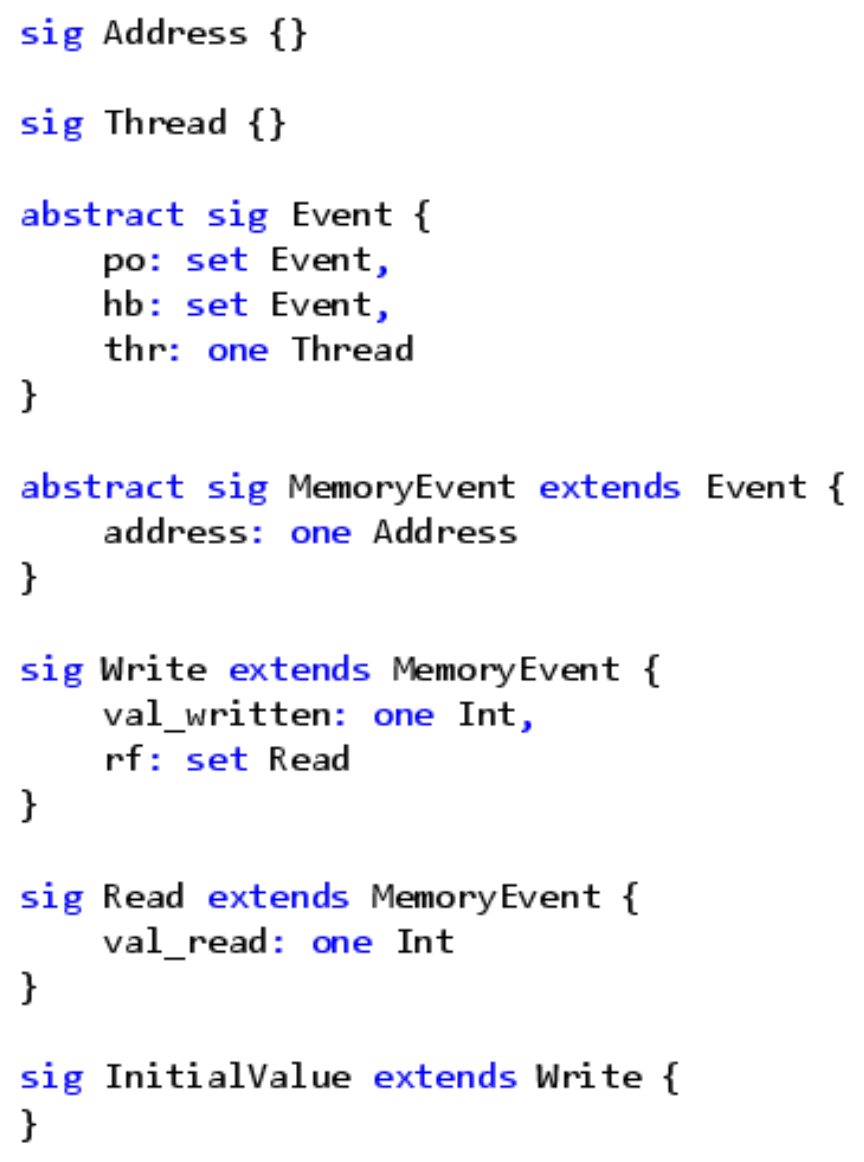
\includegraphics[width=0.6\columnwidth]{assets/axiomatic_semantics}

From there we can add all the rules as constraints.


\subsection{Memory Model Evaluation \\Framework}

Based on documentation, we can build a formal Remote Memory Access (RMA) model in Alloy. Then automatically generate tests, together with their allowed executions by the formal RMA model. After running the tests on real RMA networks we can compare the real executions with executions allowed by the model.
\begin{center}
	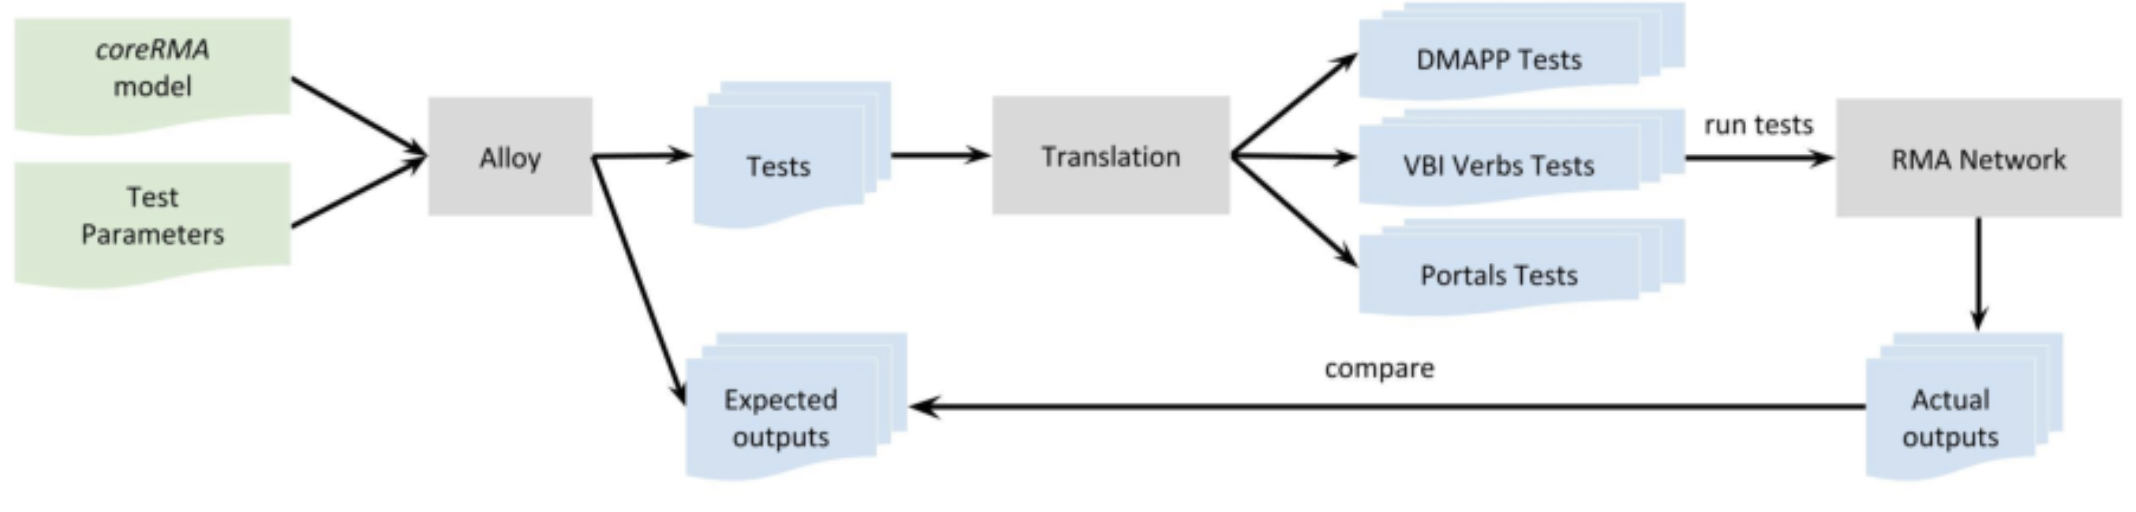
\includegraphics[width=\columnwidth]{assets/coreRMA}
\end{center}
